%! TEX root = ../final-project.tex
\chapter{ANALISIS PERMASALAHAN DAN RANCANGAN SOLUSI}

\section{Analisis Permasalahan}
\label{section:permasalahan}

Standar ARINC 653 berfungsi sebagai panduan pengembangan sistem operasi \textit{real-time} pada
\textit{safety-critical system}. Banyak faktor yang menentukan apakah sebuah sistem dapat
dikategorikan sebagai \textit{safety-critical system}, salah satunya adalah
\textit{fault-tolerancy}.  Pada \textit{safety\hyp critical system}, \textit{fault-tolerant}
adalah properti yang sangat dicari. Sistem yang \textit{fault-tolerant} akan memberikan jaminan
bahwa sistem akan terus bekerja sebagaimana seharusnya meskipun terjadi kegagalan selama
sistem beroperasi.

Fokus dari standar ARINC 653 adalah menjamin sistem operasi melakukan partisi lingkungan
eksekusi agar aplikasi yang berjalan pada sebuah lingkungan eksekusi tidak mengganggu aplikasi
pada lingkungan eksekusi lainnya. Meski standar tersebut menjamin kegagalan yang terjadi pada
sebuah aplikasi tidak akan mengganggu aplikasi lain yang berada pada lingkungan eksekusi berbeda
(\textit{fault containment}), kegagalan yang terjadi pada sebuah aplikasi tetap akan terjadi.
Standar ARINC 653 mendefinisikan mekanisme untuk mendeteksi dan memberikan tanggapan apabila
terjadi kegagalan. Namun, standar tersebut tidak mendefinisikan tanggapan apa yang harus
dilakukan untuk menjamin aplikasi yang ditangani tidak akan mengalami kegagalan yang sama dalam
waktu dekat. Meskipun aplikasi avionik pada umumnya akan melalui proses verifikasi untuk
menjamin tidak akan terjadi kegagalan, proses verifikasi tersebut mungkin sangat lama dan/atau
tidak berhasil melakukan pengujian pada kasus khusus yang mengakibatkan kegagalan. Karena itu,
mekanisme penanganan kegagalan tidak dapat diabaikan begitu saja.

Seperti yang telah dipaparkan pada \autoref{section:health_monitoring}, sistem ARINC 653
mengisolasi kegagalan yang terjadi pada sebuah partisi sehingga kegagalan tersebut tidak akan
memberikan efek apapun pada partisi lain. Kemudian, partisi yang mengalami kegagalan akan
terdeteksi oleh \textit{health monitor} pada sistem. \textit{Health monitor} akan melakukan
\textit{recovery action} sesuai dengan jenis kegagalan yang terjadi. Meski demikian,
\textit{recovery action} yang dispesifikasikan akan mengakibatkan partisi tidak berjalan untuk
rentang waktu tertentu dan tidak dapat mengatasi permasalahan apabila penyebab kegagalan
persisten pada partisi tersebut sehingga partisi tetap mengalami kegagalan.

Permasalahan yang terjadi apabila terdapat partisi yang tidak berjalan atau mengalami kegagalan
adalah layanan yang disediakan akan berhenti bekerja dan/atau memberikan hasil perhitungan yang
salah. Dalam avionika, hal ini dapat mengakibatkan kesalahan pada sistem kendali sehingga
meningkatkan kemungkinan terjadinya bahaya pada manusia dan lingkungan.

\section{Rancangan Solusi}
\label{section:solution}

Solusi dari permasalahan yang dipaparkan pada \autoref{section:permasalahan} adalah dengan
membuat sistem menjadi lebih andal. Untuk membuat sistem ARINC 653 menjadi lebih andal, salah
satu solusi yang telah dipelajari sebelumnya adalah dengan menggunakan \textit{primary-backup
scheduling} pada \textit{hierarchical scheduler} \citep{Campbell1986} \citep{Bertossi2006}.
Penggunaan skema \textit{primary-backup} dapat menjamin apabila partisi mengalami kegagalan,
maka akan terdapat partisi \textit{backup} yang dapat menyediakan layanan tersebut. Dengan
demikian, layanan tidak akan mengalami \textit{fault} dalam waktu panjang.  Namun, meski sudah
banyak studi mengenai \textit{primary-backup scheduling} pada \textit{hierarchical scheduler},
belum ada studi penggunaan \textit{primary-backup scheduling} spesifik pada sistem ARINC 653 dan
belum ada implementasi sistem ARINC 653 dengan menggunakan \textit{primary-backup scheduling}
yang tersedia secara gratis.

\textit{Primary-backup scheduling} hanya akan diterapkan pada \textit{partition scheduler}. Hal
ini dikarenakan \textit{process scheduler} bergantung pada sistem yang digunakan oleh partisi.
Agar solusi dapat bekerja untuk kasus umum, solusi yang ditawarkan harus merupakan solusi yang
tidak bergantung pada \textit{process scheduler}, dengan asumsi mekanisme \textit{process scheduler}
yang digunakan tetap sesuai spesifikasi pada standar ARINC 653.

Dengan menggunakan \textit{primary-backup}, layanan yang diberikan oleh partisi yang mengalami
kegagalan akan tetap dapat berjalan dengan memberikan kuantum waktu CPU pada partisi \textit{backup}.
Skema umum \textit{primary-backup} akan membuat \textit{backup} tersebut identik dengan partisi
\textit{primary}. Meski skema tersebut dapat membuat sistem terlihat tidak pernah mengalami
kegagalan sama sekali, partisi yang identik berarti kegagalan yang terjadi pada partisi
\textit{primary} cepat atau lambat akan terjadi pada partisi \textit{backup}.

Agar sistem yang menggunakan \textit{primary-backup partition scheduling} dapat berjalan secara
terus menerus, partisi \textit{backup} tidak harus merupakan partisi yang identik dengan partisi
\textit{primary}. Partisi \textit{backup} cukup memberikan layanan yang identik dengan layanan
yang diberikan oleh partisi \textit{primary}. Layanan tersebut dapat berupa aplikasi dengan
versi yang sudah terbukti lebih stabil, meski tidak seoptimal layanan dengan versi baru. Solusi
ini mencakup kemungkinan yang lebih umum ketimbang partisi \textit{backup} yang identik.

Implementasi dan pengujian \textit{primary-backup partition scheduling} akan dilakukan pada
ARLX, yaitu prototipe sistem yang bersesuaian dengan spesifikasi ARINC 653 pada Xen. Hal ini
dikarenakan prototipe tersebut tersedia gratis dan \textit{open-source}, sehingga penelitian
maupun pengembangan terkait dengan sistem ARINC 653 tidak memerlukan biaya banyak dan mudah
untuk mengembangkan komponen baru.

\subsection{Implementasi \textit{Primary-Backup Partition Scheduling} pada ARLX}

Pada ARLX, pembuatan sebuah partisi membutuhkan waktu yang cukup lama. Agar partisi
\textit{backup} dapat langsung menggantikan partisi \textit{primary} ketika mengalami mengalami
kegagalan, maka partisi \textit{backup} sudah harus dibuat pada tahap inisialisasi atau sistem.

\textit{Scheduler} membutuhkan daftar jadwal layanan-layanan yang akan disediakan pada setiap
\textit{major time frame}. \textit{Scheduler} akan mendapatkan daftar jadwal layanan melalui
\textit{hypercall}. Kemudian, \textit{scheduler} akan memilih partisi yang akan diberi kuantum
waktu CPU. Partisi hanya akan diberikan kuantum waktu CPU jika partisi tersebut tidak mengalami
kegagalan.

Selain itu, \textit{scheduler} juga perlu mengetahui kapan sebuah partisi \textit{primary}
dikategorikan mengalami kegagalan. Oleh karena itu, perlu ada mekanisme untuk mendeteksi
\textit{fault}, dan memberikan informasi tersebut kepada \textit{scheduler}.

\subsection{Daftar Jadwal}
\label{section:daftar_jadwal}

\textit{Partition scheduler} akan bekerja pada sebuah daftar jadwal yang terdapat pada konteks
global milik \textit{scheduler}. Dengan demikian, informasi tersebut dapat diakses kapan pun
apabila dibutuhkan oleh \textit{scheduler}. Daftar jadwal dapat diberikan oleh \textit{user
space} melalui \textit{hypercall} yang disediakan. Setiap perubahan yang terjadi pada
\textit{daftar jadwal} akan mengakibatkan seluruh proses penjadwalan yang sedang dilakukan oleh
\textit{scheduler} diulang kembali. Dengan demikian, daftar jadwal sebaiknya hanya dilakukan
pada saat pengaturan awal dan tidak dilakukan pada saat sistem sedang bekerja pada lingkungan
produksi.

\begin{figure}[h]
	\centering
	\begin{tikzpicture}[
		base/.style={scale=0.9, draw, text opacity=1.0},
		block/.style={base, text centered, minimum size=45pt}
	]
	
	\foreach \x in {0,...,4}{
		\node[block] at (45pt*\x,0) (\x) {$E_\x$};
	}
	
	\node[base, minimum height=65pt, minimum width=120pt, text width=120pt] at
		(45pt*2,-110pt) (zoomed) {
			Entri $E_2$
			\begin{itemize}
				\item \texttt{service id}
				\item \texttt{address $P$}
				\item \texttt{runtime}
			\end{itemize}
		};
	\draw[->, thick, dashed] (2) -- (zoomed);
	\node at (12pt, 33pt) (label) {Daftar Jadwal};
	\node[draw, rounded corners, inner sep=10pt] (schedlist) [fit = (0) (1) (2) (3) (4)
		(label)] {};
	\end{tikzpicture}

	\vspace{20pt}

	\caption{Daftar jadwal layanan}
	\label{figure:daftar_jadwal}
\end{figure}

Daftar jadwal berupa sebuah struktur data \textit{array}. Masing-masing elemen pada
\textit{array} tersebut disebut sebagai sebuah entri. Setiap entri akan memiliki informasi
berupa batasan \textit{real-time} layanan tersebut beserta penunjuk yang mengarah pada daftar
partisi-partisi yang akan menyediakan layanan tersebut apabila diberikan kuantum waktu CPU. Dengan
demikian, pada saat \textit{scheduler} sedang memproses sebuah layanan, \textit{scheduler} dapat
memilih partisi yang akan dijalankan dengan cepat. Setiap entri hanya akan memiliki sebuah
daftar partisi yang dapat menyediakan layanan, sehingga entri dapat dikatakan menunjuk pada
daftar penyedia layanan. Ilustrasi daftar jadwal dapat dilihat pada
\autoref{figure:daftar_jadwal}.

\subsection{Informasi Partisi}
\label{section:informasi_partisi}

Agar skema \textit{primary-backup} dapat dilakukan, \textit{scheduler} harus mengetahui beberapa
informasi terkait keadaan partisi agar dapat menentukan partisi mana yang harus mendapatkan
kuantum waktu CPU. \textit{Scheduler} harus mengetahui apakah partisi tersebut mengalami kegagalan atau
tidak. Apabila partisi sedang mengalami kegagalan, maka partisi tidak boleh mendapatkan jatah
kuantum waktu CPU. Selain itu, \textit{scheduler} juga harus mengetahui layanan apa saja yang sudah
dikerjakan sebelumnya pada \textit{major time frame} saat ini. Dengan demikian, partisi yang
memiliki layanan yang tidak bersifat \textit{idempotent} tidak akan mendapatkan kuantum waktu CPU lebih
dari sekali.

\begin{figure}[h]
	\centering
	\begin{tikzpicture}[
		base/.style={draw, text opacity=1.0, rounded corners, minimum width=55pt,
		minimum height=35pt, font=\scriptsize},
		arrow/.style={font=\tiny, midway, above, text width=50pt},
		userspace/.style={},
		kernelspace/.style={},
		partition/.style={base, userspace},
		xl/.style={base, userspace},
		hypervisor/.style={base, kernelspace},
		scheduler/.style={base, kernelspace},
		sep/.style={draw, dashed, inner sep=30pt}
		]

		\node[partition] (partisi) {Partisi};
		\node[xl, below of=partisi, yshift=-50pt] (xl)  {xl};
		\node[hypervisor, right of=xl, xshift=150pt] (hypervisor) {Hypervisor};
		\node[scheduler, above of=hypervisor, yshift=50pt] (scheduler) {Scheduler};

		\draw[->] (partisi) -- node[arrow, anchor=east] {mengirimkan informasi partisi} (xl);
		\draw[->] (xl) -- node[arrow] {mengirimkan IRQ} (hypervisor);
		\draw[->] (hypervisor) -- node[arrow, anchor=west] {memanggil \textit{handler}} (scheduler);

		\node [above of=partisi, font=\scriptsize] (uslabel){User Space};
		\node [above of=scheduler, font=\scriptsize] (hylabel) {Hypervisor};
		\node [sep] (ussep) [fit = (partisi) (xl) (uslabel)] {};
		\node [sep] (hysep) [fit = (hypervisor) (scheduler) (hylabel)] {};

	\end{tikzpicture}

	\vspace{20pt}
	\caption{Alur informasi sistem}
	\label{figure:alur_informasi}
\end{figure}

Informasi mengenai keadaan partisi dapat disimpan dengan menggunakan \textit{boolean}. Informasi
mengenai identifikasi layanan yang terdapat pada partisi dapat disimpulkan berdasarkan daftar
jadwal yang didapat melalui \textit{hypercall} seperti yang telah dipaparkan pada
\autoref{section:daftar_jadwal}. Apabila sebuah partisi $P$ berada pada rentang waktu milik
layanan $A$, maka partisi $P$ diasumsikan menyediakan layanan $A$. Alur pengiriman informasi
dapat dilihat pada \autoref{figure:alur_informasi}.

\subsection{Algoritma \textit{Scheduling}}
\label{section:algoritma_scheduling}

Algoritma \textit{scheduling} pada sistem \textit{real-time} harus deterministik agar
administrator sistem dapat mengatur konfigurasi proses-proses \textit{real-time} sehingga
memenuhi batasan-batasan masing-masing proses. Agar algoritma \textit{scheduling} tetap
deterministik, algoritma tersebut harus tidak bergantung pada sumber eksternal. Dengan demikian,
algoritma \textit{primary-backup scheduling} yang dibuat harus secara penuh bergantung kepada
informasi masing-masing partisi. \textit{Scheduler} akan memberikan kuantum waktu CPU kepada partisi
yang tidak sedang mengalami kegagalan dan layanan tersebut belum pernah
disediakan. Sebuah layanan dikatakan belum pernah disediakan jika dan hanya jika dan
hanya jika tidak ada partisi dengan layanan yang sama dengan layanan partisi
tersebut yang sudah diberikan kuantum waktu CPU pada suatu \textit{major time frame}.

\begin{figure}
	\begin{tikzpicture}[
		base/.style={scale=0.9, draw, text opacity=1.0, font=\tiny, text width=35pt},
		block/.style={base, rounded corners, text centered},
		decision/.style={base, diamond, inner sep=0pt, text badly centered},
		label/.style={scale=0.9, font=\tiny, near start},
	]

	\node[block] (mulai) {Mulai};
	\node[decision, below of=mulai, yshift=-20pt] (cek-konfigurasi) {Konfigurasi Penjadwalan Tersedia?};
	\node[block, right of=cek-konfigurasi, xshift=30pt] (mulai-major) {Mulai Major Time Frame Baru};
	\node[decision, right of=mulai-major, xshift=25pt] (cek-major) {Major Time Frame Habis?};
	\node[decision, right of=cek-major, xshift=30pt]  (cek-layanan) {Terdapat Layanan Berikutnya?};
	\node[block, right of=cek-layanan, xshift=30pt] (layanan-berikut) {Layanan Berikutnya};
	\node[decision, right of=layanan-berikut, xshift=30pt] (cek-provider) {Terdapat Penyedia Layanan Berikutnya?};
	\node[block, below of=cek-provider, yshift=-50pt] (provider-layanan) {Mendapatkan Penyedia Layanan};
	\node[decision, below of=provider-layanan, yshift=-50pt] (cek-gagal) {Partisi Penyedia Mengalami Kegagalan?};
	\node[block, right of=cek-gagal, xshift=50pt] (partisi-tidak-jalan) {Partisi Tidak Diberi Kuantum Waktu CPU};
	\node[block, left of=cek-gagal, xshift=-50pt] (partisi-jalan) {Partisi Diberi Kuantum Waktu CPU};
	\node[block, left of=partisi-jalan, xshift=-40pt] (partisi-kuantum) {Partisi Menggunakan Kuantum};
	\node[decision, left of=partisi-kuantum, xshift=-40pt] (cek-kuantum) {Kuantum Habis?};
	\node[block, above of=mulai-major, yshift=30pt] (akhir-major) {Akhir dari Major Time Frame};
	\node[block, above of=cek-layanan, yshift=30pt] (idle) {Idle};
	
	\draw[->] (mulai) -- (cek-konfigurasi);
	\draw[->] (cek-konfigurasi) -- node[label, anchor=south] {ya} (mulai-major);
	\draw[->] (cek-konfigurasi) |- ++(-30pt,-30pt) |- node[label, anchor=north, above,
		sloped] {tidak} (cek-konfigurasi);
	\draw[->] (mulai-major) -- (cek-major);
	\draw[->] (cek-major) |- node[label, anchor=west, above, sloped] {ya} (akhir-major);
	\draw[->] (cek-layanan) -- node[label, anchor=west, above, sloped] {tidak} (idle);
	\draw[->] (akhir-major) -- (mulai-major);
	\draw[->] (cek-major) -- node[label, near start, above, sloped] {tidak} (cek-layanan);
	\draw[->] (cek-layanan) -- node[label, anchor=south] {ya} (layanan-berikut);
	\draw[->] (layanan-berikut) -- (cek-provider);
	\draw[->] (cek-provider) -- ++(40pt,0pt) |- node[label, near start, above, sloped] {ya} (provider-layanan);
	\draw[->] (provider-layanan) -- (cek-gagal);
	\draw[->] (cek-provider) -- ++(0pt, -30pt) -| node[label, anchor=south] {tidak} (cek-layanan);
	\draw[->] (partisi-kuantum) -- (cek-kuantum);
	\draw[->] (cek-gagal) -- node[label, above] {tidak} (partisi-jalan);
	\draw[->] (cek-gagal) -- node[label, above] {ya} (partisi-tidak-jalan);
	\draw[->] (cek-kuantum) -- ++(0pt, -30pt) -| node[label, anchor=south] {tidak} (partisi-kuantum);
	\draw[->] (idle) -- (akhir-major);
	\draw[->] (cek-kuantum) -- ++(0pt, 60pt) -| node[label, above, sloped] {ya} (cek-major);
	\draw[->] (partisi-tidak-jalan) -- ++(0pt, 190pt) -| (cek-provider);
	\draw[->] (partisi-jalan) -- (partisi-kuantum);
	
	\end{tikzpicture}
	
	\vspace{20pt}
	\caption{Diagram \textit{Flowchart} Algoritma \textit{Scheduling}}
	\label{figure:flowchart_algoritma}
\end{figure}

Algoritma yang akan digunakan untuk melakukan \textit{scheduling} digambarkan seperti pada
\autoref{figure:flowchart_algoritma}. Scheduler akan menunggu daftar layanan yang akan
disediakan pada sebuah \textit{major time frame}. Apabila \textit{scheduler} telah mendapatkan
daftar layanan tersebut, \textit{scheduler} akan membuat \textit{major time frame} baru. Setelah
membuat \textit{major time frame} baru, \textit{scheduler} akan memilih layanan yang akan
disediakan.

Pada saat partisi akan menyediakan sebuah layanan $S$, maka \textit{scheduler} akan mendapatkan
entri $E_S$ dari daftar jadwal. Kemudian \textit{scheduler} akan memilih salah satu partisi yang
terdapat pada daftar penyedia layanan $P$ yang ditunjuk oleh entri $E_S$.  Setiap partisi
memiliki informasi partisi seperti yang telah dijelaskan pada
\autoref{section:informasi_partisi}. Dengan demikian \textit{scheduler} dapat menentukan apakah
partisi $P_i$ siap untuk diberi kuantum waktu CPU atau tidak. 

Jika partisi $P_1$ tidak siap untuk diberi kuantum waktu CPU, maka \textit{scheduler} akan mengecek
partisi $P_2$, jika partisi $P_2$ tidak siap untuk diberi kuantum waktu CPU, \textit{scheduler} akan
mengecek partisi $P_3$, dan seterusnya.  Apabila tidak terdapat partisi pada $P$ yang tidak
mengalami kegagalan, maka \textit{scheduler} akan menunggu sampai waktu pada entri $E_S$ habis
dan akan mengambil entri berikutnya.  Apabila terdapat partisi pada daftar penyedia layanan $P$
yang tidak sedang mengalami kegagalan, maka partisi tersebut akan diberi kuantum waktu CPU.  Pada saat
waktu yang diberikan sudah habis, maka \textit{scheduler} akan mengambil entri berikutnya.

\textit{Scheduler} akan menghabiskan entri layanan dan menunggu sampai periode \textit{major
frame} tersebut habis. Kemudian, \textit{scheduler} akan membuat \textit{major time frame} baru
dan mengulangi proses yang sama.  Algoritma ini akan dilakukan secara terus menerus selama
sistem berjalan.

\begin{figure}[ht]
	\centering
	\begin{tikzpicture}[
		partition-done/.style={fill=gray, fill opacity=0.50, text opacity=1.0},
		partition-healthy/.style={fill opacity=0.30, text
		opacity=1.0},
		partition-failed/.style={pattern=north west lines, fill opacity=0.40, text opacity=1.0},
		candidate/.style={very thick},
		]

		\def\boxs{30pt}
		\def\legends{10pt}
		\def\off{10pt}
		\def\loff{2pt}
		\def\xoff{15pt}
		\def\shape{rectangle +(\boxs,\boxs)}
		\def\partnode{node[pos=0.5,font=\small]}
		\def\lshape{rectangle +(\legends,\legends)}
		\newcommand\lnode[1]{node[pos=0.5,align=right,label={[anchor=west,font=\footnotesize]right:#1}] {}}

		\draw[partition-healthy]           (0*\boxs,{0*(-\boxs-\off)}) \shape \partnode {P1-SA};
		\draw[partition-healthy]           (1*\boxs,{0*(-\boxs-\off)}) \shape \partnode {P2-SA};
		\draw[partition-failed]            (2*\boxs,{0*(-\boxs-\off)}) \shape \partnode {P3-SB};
		\draw[partition-healthy]           (3*\boxs,{0*(-\boxs-\off)}) \shape \partnode {P4-SB};
		\draw[partition-healthy]           (4*\boxs,{0*(-\boxs-\off)}) \shape \partnode {P5-SB};

		\draw[partition-healthy,candidate] (0*\boxs,{1*(-\boxs-\off)}) \shape \partnode {P1-SA};
		\draw[partition-healthy]           (1*\boxs,{1*(-\boxs-\off)}) \shape \partnode {P2-SA};
		\draw[partition-failed]            (2*\boxs,{1*(-\boxs-\off)}) \shape \partnode {P3-SB};
		\draw[partition-healthy]           (3*\boxs,{1*(-\boxs-\off)}) \shape \partnode {P4-SB};
		\draw[partition-healthy]           (4*\boxs,{1*(-\boxs-\off)}) \shape \partnode {P5-SB};

		\draw[partition-done]              (0*\boxs,{2*(-\boxs-\off)}) \shape \partnode {P1-SA};
		\draw[partition-done,candidate]    (1*\boxs,{2*(-\boxs-\off)}) \shape \partnode {P2-SA};
		\draw[partition-failed]            (2*\boxs,{2*(-\boxs-\off)}) \shape \partnode {P3-SB};
		\draw[partition-healthy]           (3*\boxs,{2*(-\boxs-\off)}) \shape \partnode {P4-SB};
		\draw[partition-healthy]           (4*\boxs,{2*(-\boxs-\off)}) \shape \partnode {P5-SB};

		\draw[partition-done]              (0*\boxs,{3*(-\boxs-\off)}) \shape \partnode {P1-SA};
		\draw[partition-done]              (1*\boxs,{3*(-\boxs-\off)}) \shape \partnode {P2-SA};
		\draw[partition-failed,candidate]  (2*\boxs,{3*(-\boxs-\off)}) \shape \partnode {P3-SB};
		\draw[partition-healthy]           (3*\boxs,{3*(-\boxs-\off)}) \shape \partnode {P4-SB};
		\draw[partition-healthy]           (4*\boxs,{3*(-\boxs-\off)}) \shape \partnode {P5-SB};

		\draw[partition-done]              (0*\boxs,{4*(-\boxs-\off)}) \shape \partnode {P1-SA};
		\draw[partition-done]              (1*\boxs,{4*(-\boxs-\off)}) \shape \partnode {P2-SA};
		\draw[partition-failed]            (2*\boxs,{4*(-\boxs-\off)}) \shape \partnode {P3-SB};
		\draw[partition-healthy,candidate] (3*\boxs,{4*(-\boxs-\off)}) \shape \partnode {P4-SB};
		\draw[partition-healthy]           (4*\boxs,{4*(-\boxs-\off)}) \shape \partnode {P5-SB};

		\draw[partition-done]              (0*\boxs,{5*(-\boxs-\off)}) \shape \partnode {P1-SA};
		\draw[partition-done]              (1*\boxs,{5*(-\boxs-\off)}) \shape \partnode {P2-SA};
		\draw[partition-done]              (2*\boxs,{5*(-\boxs-\off)}) \shape \partnode {P3-SB};
		\draw[partition-done]              (3*\boxs,{5*(-\boxs-\off)}) \shape \partnode {P4-SB};
		\draw[partition-done,candidate]    (4*\boxs,{5*(-\boxs-\off)}) \shape \partnode {P5-SB};

		\draw[partition-done]              (0*\boxs,{6*(-\boxs-\off)}) \shape \partnode {P1-SA};
		\draw[partition-done]              (1*\boxs,{6*(-\boxs-\off)}) \shape \partnode {P2-SA};
		\draw[partition-done]              (2*\boxs,{6*(-\boxs-\off)}) \shape \partnode {P3-SB};
		\draw[partition-done]              (3*\boxs,{6*(-\boxs-\off)}) \shape \partnode {P4-SB};
		\draw[partition-done]              (4*\boxs,{6*(-\boxs-\off)}) \shape \partnode {P5-SB};

		\draw[->, thick] (5*\boxs+\xoff,\boxs) -- (5*\boxs+\xoff,{6*(-\boxs-\off)})
		node[midway, above, sloped] {waktu};

		% legends
		\draw[candidate] (0pt,{6*(-\boxs-\off)-0*(\legends+\loff)-\legends-\off}) \lshape
		\lnode{Partisi kandidat};

		\draw[partition-healthy]
		(0pt,{6*(-\boxs-\off)-1*(\legends+\loff)-\legends-\off}) \lshape
		\lnode{Partisi tidak mengalami kegagalan};

		\draw[partition-failed]
		(0pt,{6*(-\boxs-\off)-2*(\legends+\loff)-\legends-\off}) \lshape
		\lnode{Partisi mengalami gagal};

		\draw[partition-done]
		(0pt,{6*(-\boxs-\off)-3*(\legends+\loff)-\legends-\off}) \lshape
		\lnode{Layanan pada partisi telah disediakan};

	\end{tikzpicture}

	\vspace{10pt}
	\caption{Contoh \textit{primary-backup scheduling}}
	\label{figure:pb_scheduling}
\end{figure}

Illustrasi bagaimana algoritma \textit{primary-backup scheduling} pada \textit{scheduler} ARINC
653 bekerja dapat dilihat pada \autoref{figure:pb_scheduling}. Pada ilustrasi, partisi diberi
label dengan format $PX-SY$, yang berarti partisi $X$ akan menyediakan layanan $Y$ jika
diberikan kuantum waktu CPU oleh \textit{scheduler}. Pada skenario tersebut, \textit{scheduler} akan
bekerja sebagai berikut.

\begin{enumerate}

	\item Pada partisi $P1$, partisi tidak sedang mengalami kegagalan dan
		layanan $A$ belum pernah disediakan, sehingga partisi diberikan waktu
		CPU oleh \textit{scheduler}.

	\item Pada partisi $P2$, partisi tidak diberikan kuantum waktu CPU karena pada saat partisi $P1$
		sudah menghabiskan kuantumnya, layanan $A$ sudah pernah disediakan.

	\item Pada partisi $P3$, layanan pada partisi tersebut belum pernah disediakan,
		namun partisi sedang mengalami kegagalan sehingga partisi tidak diberikan waktu
		CPU.

	\item Partisi $P4$ tidak sedang mengalami kegagalan dan karena partisi $P3$ tidak diberikan
		kuantum waktu CPU, layanan $B$ belum pernah disediakan. Karena semua kondisi
		memenuhi, maka partisi P4 diberikan kuantum waktu CPU oleh \textit{scheduler}.

	\item Partisi $P5$ tidak diberikan kuantum waktu CPU karena layanan $B$ sudah pernah
		disediakan.

\end{enumerate}

Pada akhir dari \textit{major time frame}, algoritma ini menjamin setiap layanan pernah
disediakan apabila terdapat setidaknya satu partisi yang memiliki layanan tersebut yang
tidak sedang mengalami kegagalan. Algoritma ini akan berulang secara terus menerus tiap akhir
\textit{major time frame}.

\subsection{Mekanisme Penanganan Kegagalan}

Penanganan kegagalan dengan menggunakan \textit{primary-backup scheduler} dilakukan dengan
mengubah nilai keadaan sebuah partisi dengan menggunakan \textit{hypercall}. \textit{Hypercall}
tersebut tersedia pada dom0. \textit{Hypercall} tersebut tidak dapat diakses oleh partisi yang
terdapat pada sistem. Partisi pada sistem dapat mengatasi permasalahan tersebut dengan
menggunakan API yang tersedia pada dom0. Namun, pada penelitian ini, API tersebut tidak akan
diimplementasikan dan perubahan nilai keadaan akan dilakukan secara manual.

Sama seperti pada spesfikasi ARINC 653, metode pendeteksian kegagalan dapat dilakukan seperti
yang telah dipaparkan pada \autoref{section:health_monitoring}. Namun, pada saat menggunakan
\textit{primary-backup scheduler}, \textit{recovery action} yang dilakukan oleh sistem operasi
adalah mengubah nilai keadaan sebuah partisi.

\section{Rancangan Pengujian}
\label{section:rancangan_pengujian}

Untuk menjamin \textit{scheduler} yang dibahas pada \autoref{section:solution} dapat bekerja
sebagaimana seharusnya, perlu dilakukan pengujian terkait fungsionalitas \textit{scheduler}.
Berikut adalah fungsionalitas sistem yang akan diukur pada saat menggunakan
\textit{primary-backup partition scheduler}.

\begin{enumerate}
	\item Keandalan sistem
	\item \textit{Latency} layanan pada sistem
\end{enumerate}

Pengukuran kedua fungsionalitas tersebut dilakukan guna mencapai tujuan yang telah dipaparkan
pada \autoref{section:tujuan}. Pengukuran keandalan sistem diperlukan untuk mengkuantifikasi
peningkatan keandalan yang diakibatkan oleh penggunaan \textit{primary-backup partition
scheduler}.  Pengukuran \textit{latency} layanan pada sistem diperlukan untuk melihat efek
penggunaan \textit{primary-backup partition scheduler} pada kinerja sistem ARINC 653. Kedua
jenis pengujian tersebut akan mengumpulkan data dengan melakukan \textit{timing}, yaitu
pengukuran waktu yang terlewat dari satu titik tertentu pada masa lampau. Data tersebut kemudian
akan dianalisa untuk melihat perilaku dan kinerja dari sistem. Berdasarkan data tersebut,
kinerja sistem dapat dianggap baik apabila sistem dapat dikategorikan sebagai sistem
\textit{real-time} seperti yang telah dipaparkan pada \autoref{section:sistem_realtime}.

Perangkat lunak akan dibangun dengan menggunakan bahasa pemrograman C dan berjalan pada
\textit{user space}. Dengan demikian, hasil pengukuran yang didapat memuat \textit{delay} yang
diakibatkan oleh pemindahan data melalui \textit{system call} ketika akan meminta nilai waktu
yang dicatat oleh sistem operasi. Namun, hal tersebut diperlukan karena beberapa alasan yang
akan dipaparkan pada \autoref{section:pengujian_keandalan} dan
\autoref{section:pengujian_latency}.

\subsection{Pengujian Keandalan}
\label{section:pengujian_keandalan}
Untuk mengukur peningkatan keandalan sistem akibat penggunaan \textit{primary-backup partition
scheduler}, sistem akan menjalani pengujian keandalan pada saat menggunakan \textit{scheduler}
tersebut.  Tujuan utama dari pengujian keandalan adalah untuk mengukur \textit{mean time to
failure} sistem setelah menggunakan \textit{scheduler} tersebut. Untuk mempermudah pengukuran,
asumsikan bahwa sistem akan selalu mengalami kegagalan apabila terdapat sebuah layanan pada
sistem tersebut yang mengalami kegagalan dan layanan-layanan merupakan komponen paling tidak
andal pada sistem. Dengan demikian, \textit{mean time to failure} sistem sama dengan minimum
dari \textit{mean time to failure} seluruh layanan yang terdapat pada sistem tersebut. Keandalan
sistem dikatakan meningkat saat menggunakan \textit{primary-backup scheduler} apabila
\textit{mean time to failure} sistem tersebut menjadi lebih lama. Selain itu, hasil pengujian
dapat digunakan untuk menentukan apakah algoritma bekerja seperti yang seharusnya.

Pengujian keandalan dilakukan dengan melakukan pengecekan apakah setiap partisi dapat
mengirimkan \textit{heartbeat} dengan baik. Sebuah partisi dikatakan dapat mengirim
\textit{heartbeat} apabila partisi mengirimkan \textit{heartbeat} jika dan hanya jika partisi
tersebut memenuhi kondisi untuk mendapatkan kuantum waktu CPU. Cara termudah untuk melakukan
pengujian tersebut adalah dengan menggunakan kerangka uji dengan arsitektur
\textit{server-client} seperti pada \autoref{figure:server_client_testing_arch}.

Setiap partisi berlaku sebagai \textit{client} pada arsitektur tersebut. \textit{Server} dapat
berupa komputer apa pun yang terhubung dengan seluruh partisi menggunakan kanal TCP. TCP dipilih
karena kerangka uji didesain agar dapat digunakan antar komputer sehingga memerlukan komunikasi
antara komputer melalui jaringan. Selain itu, protokol komunikasi dipilih menggunakan TCP karena
protokol TCP menjamin paket yang dikirim akan sampai pada tujuan. Untuk mempermudah pengujian,
mesin yang digunakan untuk \textit{server} adalah dom0 pada sistem. Pada awalnya, dom0 akan
menggunakan \textit{hypercall} untuk mengubah penjadwalan partisi-partisi pada sistem sesuai
dengan skenario yang ditentukan.  Kemudian, setiap partisi mengirimkan \textit{heartbeat} dengan
selang waktu tertentu kepada \textit{server}.  Kemudian, \textit{server} akan mencatat setiap
layanan sudah pernah disediakan pada tiap akhir \textit{major time frame}. Pada saat pengujian
tersebut dijalankan, dom0 akan memanggil \textit{hypervisor} secara acak untuk mengubah keadaan
salah satu partisi. Ilustrasi langkah-langkah pengujian dapat dilihat pada
\autoref{figure:server_client_testing_impl}.

\begin{figure}[!ht]
	\centering
	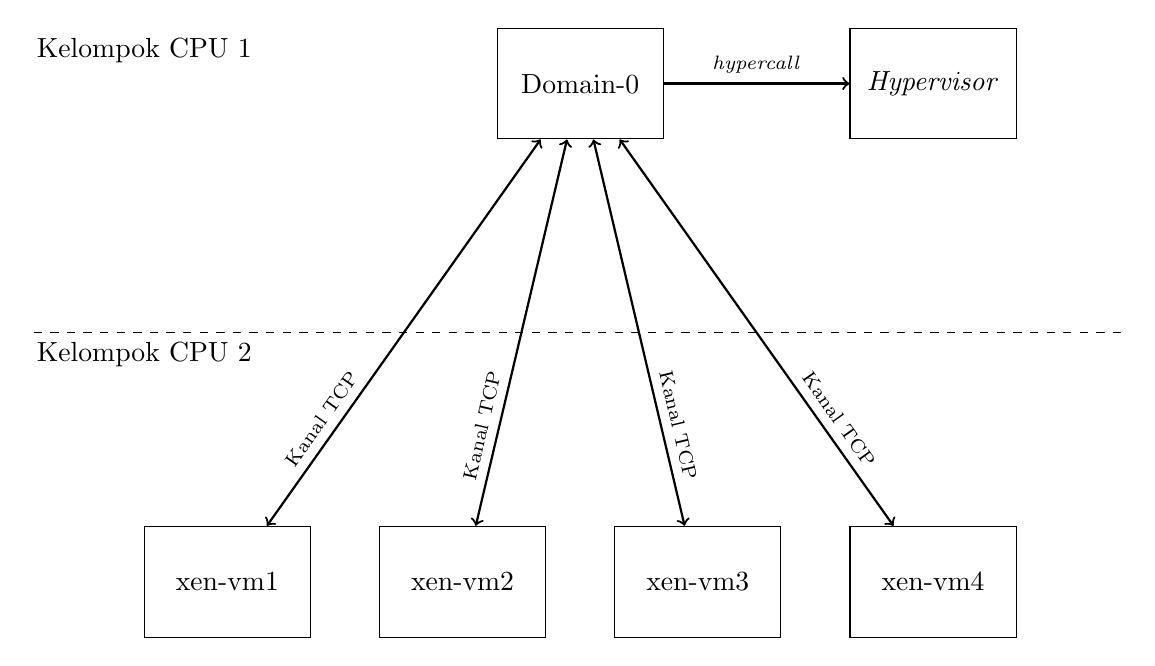
\begin{tikzpicture}[
		base/.style={draw, minimum width=60pt, minimum height=40pt},
		link/.style={<->, draw, thick}
	]

	\node[base] at (85pt*3/2, 0pt) (server) {Domain-0};
	\node[base] at (255pt, 0pt) (hypervisor) {\textit{Hypervisor}};
	\draw[->, draw, thick] (server) -- node [sloped, midway, above, font=\scriptsize] {\textit{hypercall}}(hypervisor);

	\foreach \x in {1,...,4}{
		\node[base] at ({85pt*(\x-1)}, -180pt) (\x) {xen-vm\x};
		\draw[link] (\x) -- node [sloped, near start, above, font=\scriptsize] {Kanal TCP} (server);
	}

	\draw[dashed] (-70pt,-90pt) --  (85pt*3+70pt,-90pt);

	\node at (-30pt, 20pt) [below] {Kelompok CPU 1};
	\node at (-30pt, -90pt) [below] {Kelompok CPU 2};
	
	\end{tikzpicture}
	\vspace{20pt}
	\caption{Arsitektur sistem pengujian keandalan layanan}
	\label{figure:server_client_testing_arch}
\end{figure}

Agar pengujian keandalan tersebut dapat bekerja sebagaimana seharusnya, maka batasan-batasan
berikut harus terpenuhi pada saat melakukan pengujian.

\begin{enumerate}

	\item Selang waktu harus dipilih sedemikian sehingga setiap partisi akan memberikan
		layanan tersebut apabila mendapatkan kuantum waktu CPU.

	\item \textit{Server} dan \textit{client} tidak boleh menggunakan CPU yang sama. Hal ini
		menjamin agar \textit{client} tidak mengganggu waktu eksekusi \textit{server}
		sehingga \textit{heartbeat} dari \textit{client} dapat langsung diproses oleh
		\textit{server}.
	
	\item Waktu yang digunakan untuk melakukan pengukuran pengujian adalah waktu pada
		\textit{server}. Karena waktu yang dipakai antara \textit{server} dan
		\textit{client} mungkin berbeda, perlu adanya satu sumber kebenaran waktu pada
		saat pengujian untuk menghasilkan pengukuran yang dapat terkuantifikasi.

\end{enumerate}

\begin{figure}[!ht]
	\centering
	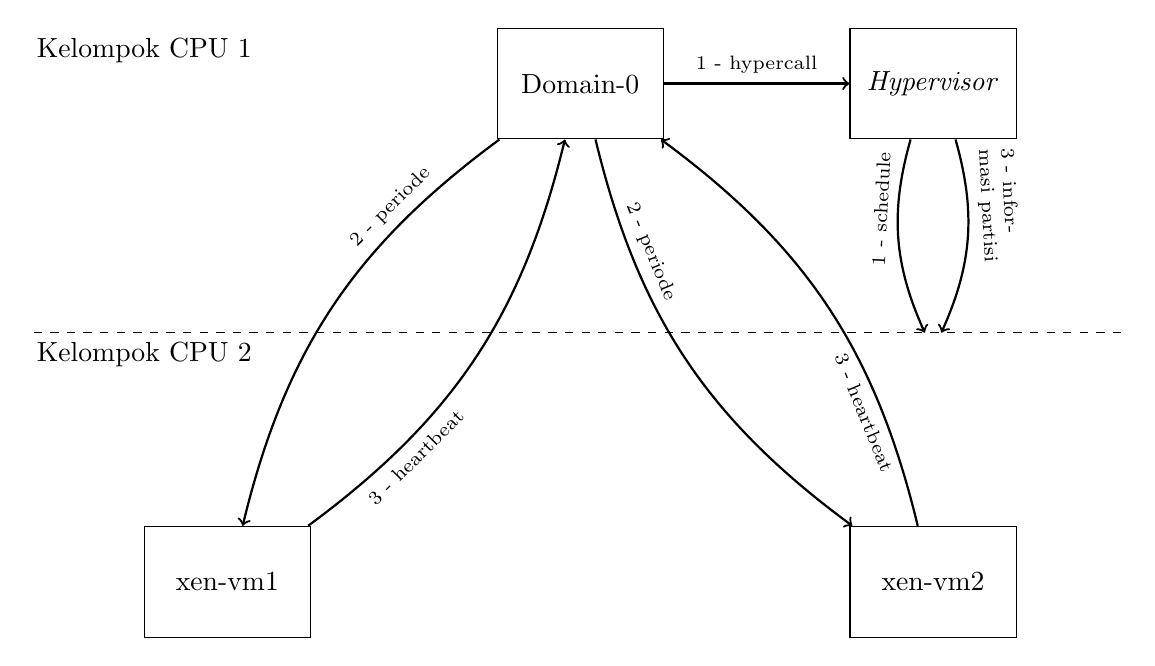
\begin{tikzpicture}[
		base/.style={draw, minimum width=60pt, minimum height=40pt},
		link/.style={->, draw, thick}
	]

	\node[base] at (85pt*3/2, 0pt) (server) {Domain-0};
	\node[base] at (255pt, 0pt) (hypervisor) {\textit{Hypervisor}};
	\draw[->, draw, thick] (server) -- node[sloped, midway, above, font=\scriptsize]
		{1 - hypercall} (hypervisor);

	\foreach \x in {1,...,2}{
		\node[base] at ({255pt*(\x-1)}, -180pt) (\x) {xen-vm\x};
		\draw[link] (\x) to[bend right=20pt] node [sloped, near start, below,
			font=\scriptsize] {3 - heartbeat} (server);
		\draw[link] (server) to[bend right=20pt] node [sloped, near start, above,
			font=\scriptsize] {2 - periode} (\x);
	}

	\draw[dashed] (-70pt,-90pt) --  (85pt*3+70pt,-90pt);

	\node at (-30pt, 20pt) [below] {Kelompok CPU 1};
	\node at (-30pt, -90pt) [below] {Kelompok CPU 2};

	\draw[->, draw, thick] (hypervisor) to[bend right=20pt] node[sloped, pos=0.35, above,
		font=\scriptsize] {1 - schedule} (252pt, -90pt);
	\draw[->, draw, thick] (hypervisor) to[bend left=20pt] node[sloped, pos=0.35, above,
		font=\scriptsize, text width=43pt]  {3 - informasi partisi} (258pt, -90pt);
	
	\end{tikzpicture}
	\vspace{20pt}
	\caption[Komunikasi pada sistem pengujian keandalan layanan]{Komunikasi pada sistem pengujian keandalan layanan sesuai dengan urutannya}
	\label{figure:server_client_testing_impl}
\end{figure}

Perlu diperhatikan bahwa penggunaan kanal TCP akan menambah \textit{delay} pada waktu hasil
pengukuran.  Ditambah dengan \textit{delay} yang diakibatkan oleh \textit{system call}, maka
hasil yang didapat memiliki resolusi waktu yang rendah.  \textit{Delay} tersebut mungkin dapat
diperkecil apabila komunikasi dilakukan menggunakan UDP. Namun, UDP tidak menjamin paket akan
sampai pada tujuan, sehingga UDP bukanlah metode komunikasi yang andal. Meski demikian, tujuan
utama pengujian keandalan dilakukan adalah untuk melihat keandalan sistem dan bukan untuk
melihat kinerja sistem. Apabila terdapat paket yang hilang, maka hasil perhitungan keandalan
sistem akan berbeda secara signifikan. Dengan demikian, kanal TCP tetap dipilih sebagai metode
komunikasi antara \textit{client} dan \textit{server} pada pengujian keandalan.

Pengujian keandalan juga dapat digunakan untuk menghitung \textit{latency} dari masing-masing
layanan. Namun, seperti yang telah dijelaskan sebelumnya, akan terdapat \textit{delay} pada
waktu hasil pengukuran dikarenakan I/O. Meski demikian, \textit{latency} yang didapat akan tetap
bermanfaat untuk melihat kinerja sistem apabila layanan yang berjalan pada partisi akan
menggunakan I/O (\textit{I/O-bound}).

\subsection{Pengujian \textit{Latency} Layanan}
\label{section:pengujian_latency}

Pengujian \textit{latency} layanan dilakukan dengan melakukan \textit{periodic task} pada
partisi-partisi yang berada pada sistem. Selisih waktu antara waktu yang seharusnya dengan waktu
ketika \textit{task} tersebut dapat diselesaikan merupakan \textit{latency} yang akan diukur
pada saat pengujian. Pengujian akan dilakukan menggunakan POSIX \textit{timer}, yaitu
\textit{system interface} yang digunakan untuk mendapatkan notifikasi pada waktu yang akan
datang dan juga secara berkala \citep{POSIX}. Pada saat \textit{task} tersebut mendapatkan waktu
CPU, \textit{task} tersebut akan langsung mencatat waktu pada saat itu. Pada saat program
pengujian selesai dijalankan, maka program tersebut akan menuliskan catatannya kedalam sebuah
\textit{file}.

Pengujian akan dilakukan pada \textit{user space} dikarenakan aplikasi yang akan dibangun pada
sistem ini akan berupa aplikasi yang berjalan pada \textit{user space} juga. Dengan demikian,
hasil pengujian diharapkan dapat memberikan gambaran perilaku sistem serta jaminan yang akan
diberikan oleh sistem apabila pengembang mengembangkan aplikasi pada sistem tersebut.

Karena pengujian \textit{latency} tidak membutuhkan komunikasi dengan partisi lain, maka
\textit{timing} dapat dilakukan tanpa membutuhkan I/O. Dengan demikian, hasil pengujian
\textit{latency} merepresentasikan kemampuan maksimal dari sistem. Selain itu, hasil pengujian
dapat dijadikan referensi pada saat membuat desain layanan yang kinerjanya berdasarkan kecepatan
CPU (\textit{CPU-bound}).

% vim: tw=96
